\documentclass[calcdimensions,landscape,letterpaper]{powersem}
\usepackage{color}
\usepackage[pdftex]{thumbpdf} % For thumbnails
\usepackage[pdftex]{hyperref} % For links.
\usepackage[display,coloremph,whitebackground]{texpower} % colormath
\usepackage{fixseminar}
\usepackage{tpslifonts}
\usepackage[pdftex,final]{graphicx} % For including graphics.
\usepackage{animate}
\usepackage[utf8]{inputenc}
\usepackage{minted}
\usepackage{amsmath}
\usepackage{amssymb}
\usepackage{eurosym}
\usepackage{booktabs} % rules in tables
\usepackage{multirow} % multi-row cells
\usepackage{rotating} % text rotation
\usepackage{tipa}

\title{The SOLID Principles}
\author{Jan Wedekind}
\date{Thursday, Feb 22nd 2022}

\DeclareGraphicsExtensions{.jpg,.pdf,.png}
\pdfcompresslevel=9

\hypersetup{
   pdftitle          = {\thetitle},
   pdfsubject        = {After Catchup Presentation 22nd Feb 2022},
   pdfauthor         = {Jan Wedekind},
   pdfkeywords       = {},
   pdfcreator        = {okular},
   pdfproducer       = {LaTeX with hyperref and thumbpdf},
   bookmarksopen     = false,
   bookmarksnumbered = true,
   colorlinks        = true,
   pdfstartpage      = {1},
   pdfpagemode       = {FullScreen}
}

% \textregistered for (R)
% \copyright for (C)
% \texttrademark for (TM) 

\DeclarePanel{top}{
  \begin{picture}(0,0)
    \put(15,-25){\parbox[c]{.8\textwidth}{\center\large\bf\thecurrentheading}}
  \end{picture}
}

\DeclarePanel{bottom}{
  \begin{picture}(0,0)
    \put(0,15){\parbox[c]{.98\pdfpagewidth}{\tiny\thedate\hfill\theslide}}
  \end{picture}
}

\slidesmag{4}
\backgroundstyle{none}
\slideframe{none}
\pagestyle{empty}

\mklength{\slideleftmargin}{-2cm}
\mklength{\sliderightmargin}{-2cm}
\mklength{\slidetopmargin}{2.0cm}
\mklength{\slidebottommargin}{1.5cm}

\renewcommand{\currentpagevalue}{\value{slide}}
\newcommand{\thecurrentheading}{}
\newcommand{\heading}[1]{\renewcommand{\thecurrentheading}{#1}}
\newcommand{\subheading}[1]{\concept{#1}}

\begin{document}

\begin{slide}
  \pdfbookmark[1]{\thetitle}{title}
  \heading{\ }
  \begin{center}
    \maketitle
  \end{center}
\end{slide}

\begin{slide}
  \pdfbookmark[1]{Motivation}{motivation}
  \heading{Motivation}
  \textbf{Me:} What is the motivation for the SOLID software design principles?\\
  \textbf{ChatGPT:} ... Overall, the SOLID principles aim to create software that is easier to understand, extend, and maintain
  over time, ultimately leading to higher quality, more robust software systems.
\end{slide}

\begin{slide}
  \pdfbookmark[1]{Software Rot}{software-rot}
  \heading{Software Rot}
  \begin{center}
    \textbf{Symptoms of rotting software design}\footnote{Robert C. Martin: Design Principles and Design Patterns}
    \begin{itemize}
      \item \textbf{Rigidity}: software difficult (a lot of work) to change
      \item \textbf{Fragility}: changes easily break the software
      \item \textbf{Immobility}: it is easier to rewrite than reuse parts
      \item \textbf{Viscosity}: design preserving methods are harder to employ than hacks
    \end{itemize}
  \end{center}
\end{slide}

\begin{slide}
  \pdfbookmark[1]{Aims of SOLID}{solid-aims}
  \heading{Aims of SOLID}
  \begin{center}
    \textbf{Aims of SOLID}\footnote{Robert C. Martin: Design Principles and Design Patterns}\medskip\\
    \begin{minipage}[c]{.65\textwidth}
      \begin{itemize}
        \item Keep software application \textbf{flexible}
        \item Keep software application \textbf{robust}
        \item Keep software application \textbf{reusable}
        \item Keep software application \textbf{developable}
      \end{itemize}
    \end{minipage}
  \end{center}
\end{slide}

\begin{slide}
  \pdfbookmark[1]{Robert C. Martin}{robertmartin}
  \heading{Robert C. Martin aka "Uncle Bob"}
  \begin{center}
    \begin{minipage}[c]{.4\textwidth}
      \begin{center}
        \resizebox*{.93\textwidth}{!}{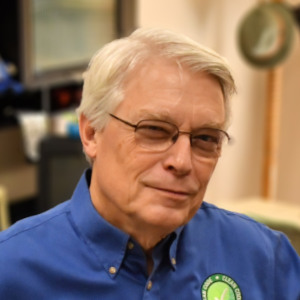
\includegraphics{robert-martin}}\\
        Robert C. Martin
      \end{center}
    \end{minipage}
    \begin{minipage}[c]{.55\textwidth}
      \begin{itemize}
        \item Born 5.12.1952
        \item One of \href{https://agilemanifesto.org/}{Agile Manifesto}'s authors
        \item Author of \href{https://www.informit.com/store/clean-code-a-handbook-of-agile-software-craftsmanship-9780132350884}{Clean Code}, \href{https://www.informit.com/store/functional-design-principles-patterns-and-practices-9780138176396}{Functional Design}, and more books
        \item software consultant and trainer
        \item Author of \href{https://web.archive.org/web/20150906155800/http://www.objectmentor.com/resources/articles/Principles_and_Patterns.pdf}{Design Principles and Design Patterns} which later became SOLID
        \item Speaker at many conferences
        \item Advocate of Test-Driven Development
      \end{itemize}
    \end{minipage}
  \end{center}
\end{slide}

\begin{slide}
  \pdfbookmark[1]{The SOLID Principles}{solid-principles}
  \heading{The SOLID Principles}
  \begin{center}
    \begin{minipage}[c]{.4\textwidth}
      \begin{enumerate}
        \item \textbf{S}ingle responsibility
        \item \textbf{O}pen-closed
        \item \textbf{L}iskov substitution
        \item \textbf{I}nterface segregation
        \item \textbf{D}ependency inversion
      \end{enumerate}
    \end{minipage}
  \end{center}
\end{slide}

\begin{slide}
  \pdfbookmark[1]{Single Responsibility}{single-responsibility}
  \pdfbookmark[2]{Before}{single-responsibility-before}
  \heading{Single Responsibility - Before}
  \begin{center}
    \begin{minted}{python}
def adults_to_html(people):
    result = "<ul>\n"
    for person in people:
        if person.age >= 18:
            result += "  <li>" + person.name + "</li>\n"
    result += "</ul>"
    return result
# ...
page = adults_to_html(people)
    \end{minted}
  \end{center}
\end{slide}

\begin{slide}
  \pdfbookmark[2]{After}{single-responsibility-after}
  \heading{Single Responsibility - After}
  \begin{center}
    \begin{minted}{python}
def select_adults(people):
    return [person for person in people if person.age >= 18]

def people_to_html(people):
    result = "<ul>\n"
    for person in people:
        result += "  <li>" + person.name + "</li>\n"
    result += "</ul>"
    return result
# ...
page = people_to_html(select_adults(people))
    \end{minted}
  \end{center}
\end{slide}

\begin{slide}
  \pdfbookmark[1]{Open-Closed}{open-closed}
  \pdfbookmark[2]{Before}{open-closed-before}
  \heading{Open-Closed - Before}
  \begin{center}
    \begin{minted}{python}
def total_area(shapes):
  result = 0
  for shape in shapes:
    match type(shape):
      case Rectangle:
        result += shape.width * shape.height
      case Sphere:
        result += math.pi * shape.radius ** 2
      case _:
        raise f"Unsupported shape {shape}"
  return result
    \end{minted}
  \end{center}
\end{slide}

\begin{slide}
  \pdfbookmark[2]{After}{open-closed-after}
  \heading{Open-Closed - After}
  \begin{center}
    \begin{minted}{python}
class Rectangle:
  def area(self):
    return self.width * self.height

class Circle:
  def area(self):
    return math.pi * self.radius ** 2

def total_area(shapes):
  result = 0
  for shape in shapes:
    result += shape.area()
  return result
    \end{minted}
  \end{center}
\end{slide}

\begin{slide}
  \pdfbookmark[1]{Liskov-Substitution}{liskov-substitution}
  \pdfbookmark[2]{Before}{liskov-substitution-before}
  \heading{Liskov-Substitution - Before}
  \begin{center}
    \begin{minipage}[c]{.6\textwidth}
      \begin{minted}{python}
class Rectangle:
  def __init__(self, width, height):
    self.width = width
    self.height = height
  def set_width(self, width):
    self.width = width
  def set_height(self, height):
    self.height = height

class Square(Rectangle):
  def __init__(self, side):
    super().__init__(side, side)
      \end{minted}
    \end{minipage}
    \begin{minipage}[c]{.35\textwidth}
      \begin{center}
        \resizebox*{.93\textwidth}{!}{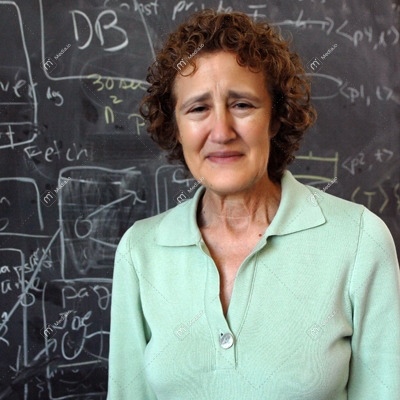
\includegraphics{liskov-depressed}}\\
        Barbara Liskov (sad)
      \end{center}
    \end{minipage}
  \end{center}
\end{slide}

\begin{slide}
  \pdfbookmark[2]{After}{liskov-substitution-after}
  \heading{Liskov-Substitution - After}
  \begin{center}
    \begin{minipage}[c]{.6\textwidth}
      \begin{minted}{python}
class Shape:
  pass

class Rectangle(Shape):
  def __init__(self, width, height):
    self.width = width
    self.height = height
  def set_width(self, width):
    self.width = width
  def set_height(self, height):
    self.height = height

class Square(Shape):
  def __init__(self, side):
    self.side = side
  def set_side(self, side):
    self.side = side
      \end{minted}
    \end{minipage}
    \begin{minipage}[c]{.35\textwidth}
      \begin{center}
        \resizebox*{.93\textwidth}{!}{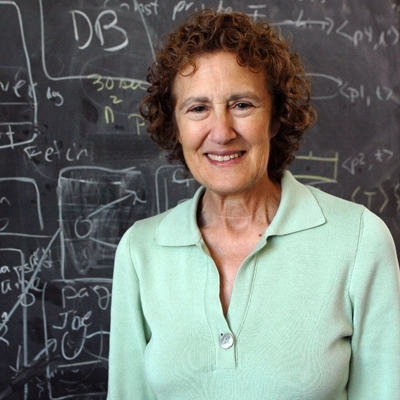
\includegraphics{barbara-liskov}}\\
        Barbara Liskov (happy)
      \end{center}
    \end{minipage}
  \end{center}
\end{slide}

\begin{slide}
  \pdfbookmark[2]{Contracts}{liskov-substitution-contracts}
  \heading{Liskov-Substitution - Contracts}
  \begin{center}
    ``The Liskov Substitution Principle states, among other constraints, that a subtype is not substitutable for its super type
    if it strengthens its operations' preconditions, or weakens its operations' postconditions''\footnote{\href{https://www.cs.ubc.ca/~ebani/papers/LiskofHappySad_ICSE-SEET_2018.pdf}{Baniassad: Making the Liskov Substitution Principle Happy and Sad}}\bigskip\\
    \resizebox*{.8\textwidth}{!}{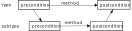
\includegraphics{liskov}}
  \end{center}
\end{slide}

\begin{slide}
  \pdfbookmark[1]{Interface Segregation}{interface-segregation}
  \pdfbookmark[2]{Before}{interface-segregation-before}
  \heading{Interface Segregation - Before}
  \begin{center}
    \begin{minted}{python}
class AccountHolder:
  def __init__(self, name, age, balance):
    self.name = name
    self.age = age
    self.balance = balance
  def is_adult(self):
    return self.adult >= 18
  def deposit(self, amount):
    self.balance += amount
  def withdraw(self, amount):
    self.balance -= amount
    \end{minted}
  \end{center}
\end{slide}

\begin{slide}
  \pdfbookmark[2]{After}{interface-segregation-after}
  \heading{Interface Segregation - After}
  \begin{center}
    \begin{minted}{python}
class Person:
  def __init__(self, name, age):
    self.name, self.age = name, age
  def is_adult(self):
    return self.adult >= 18

class Account:
  def __init__(self, balance):
    self.balance = balance
  def deposit(self, amount):
    self.balance += amount
  def withdraw(self, amount):
    self.balance -= amount

class AccountHolder(Person):
  def __init__(self, name, age, account):
    super().__init__(name, age)
    self.account = account
    \end{minted}
  \end{center}
\end{slide}

\begin{slide}
  \pdfbookmark[1]{Dependency Inversion}{dependency-inversion}
  \pdfbookmark[2]{Before}{dependency-inversion-before}
  \heading{Dependency Inversion - Before}
  \begin{center}
    \begin{minted}{python}
def get_names(connection):
    cursor = connection.cursor()
    cursor.execute('SELECT name FROM member_table')
    rows = cursor.fetchall()
    names = [row[0] for row in rows]
    return names

connection = sqlite3.connect('example.db')
names_list = get_names(connection)
connection.close()
print(names_list)
    \end{minted}
  \end{center}
\end{slide}

\begin{slide}
  \pdfbookmark[2]{After}{interface-segregation-after}
  \heading{Dependency Inversion - After}
  \begin{center}
    \begin{minted}{python}
class Database(abc.ABC):
  @abc.abstractmethod
  def get_names(self):
    pass

class SQLiteDatabase(Database):
  def __init__(self, db_file_name):
    self.connection = sqlite3.connect(db_file_name)
  def __del__(self):
    self.connection.close()
  def get_names(self):
    cursor = self.connection.cursor()
    cursor.execute('SELECT name FROM member_table')
    rows = cursor.fetchall()
    return [row[0] for row in rows]
    \end{minted}
  \end{center}
\end{slide}

\begin{slide}
  \heading{Dependency Inversion - After}
  \begin{center}
    \begin{minted}{python}
database = SQLiteDatabase('example.db')
names_list = database.get_names()
print(names_list)
    \end{minted}
  \end{center}
\end{slide}

\begin{slide}
  \pdfbookmark[1]{SOLID Overview}{solid-overview}
  \heading{SOLID Overview}
  \begin{center}
    \animategraphics[loop,autoplay,width=.65\textwidth]{8}{solidframe-}{0}{59}
  \end{center}
\end{slide}

\begin{slide}
  \pdfbookmark[1]{ArjanCodes video}{arjancodes-video}
  \heading{ArjanCodes: Uncle Bob's SOLID Principles Made Easy}
  \begin{center}
    \href{https://www.youtube.com/watch?v=pTB30aXS77U}{\resizebox*{.95\textwidth}{!}{
\includegraphics{arjancodes}}}
  \end{center}
\end{slide}

\begin{slide}
  \pdfbookmark[1]{Connascence}{connascence}
  \heading{Further Reading: Connascence}
  \textbf{Connascence} \textipa{[k@'neIs@ns]} is a software quality metric invented by Meilir Page-Jones to allow reasoning about the
  complexity caused by dependency relationships in object-oriented design much like coupling did for structured design. In software
  engineering, two components are connascent if a change in one would require the other to be modified in order to maintain the
  overall correctness of the system. In addition to allowing categorization of dependency relationships, connascence also provides
  a system for comparing different types of dependency. Such comparisons between potential designs can often hint at ways to
  improve the quality of the software.\footnote{\url{https://en.wikipedia.org/wiki/Connascence}}
\end{slide}

\end{document}
